\chapter{Design}\label{ch:design}

This section discusses the design of the system. The first part explains query
spawning and execution, the second part describes how data streams can be shared
between queries.

\section{Overall Architecture}

Our system consists of multiple components which are briefly described here.
A dataflow program submitted to run as part of the system is
called a \emph{query}. Following Timely's terminology, the execution of a query
is done by a group of \emph{worker} threads. Each worker manages the scheduling and
notification of the nodes that are part instance of the dataflow graph. 

A query is executed by one or more \emph{executors}. Each executor selected to
execute a query will fetch and invoke the query binary, ultimately spawning the
worker threads. 

All these components are managed by a process called the \emph{coordinator},
which stores the system state in the \emph{catalog}.

\section{Coordinator}

The purpose of the coordinator is to manage all components of the system. It
provides an interface for users to submit new queries and inspect the current
state of the system. In order to receive commands and report their internal state,
every executor and query process maintains a network connection to the coordinator.

Bookkeeping of the system is done by the coordinator in the catalog. The
catalog is a datastructure which contains all information about the available
executors, the running queries and their workers. 

\begin{figure}[htb]
  \centering
    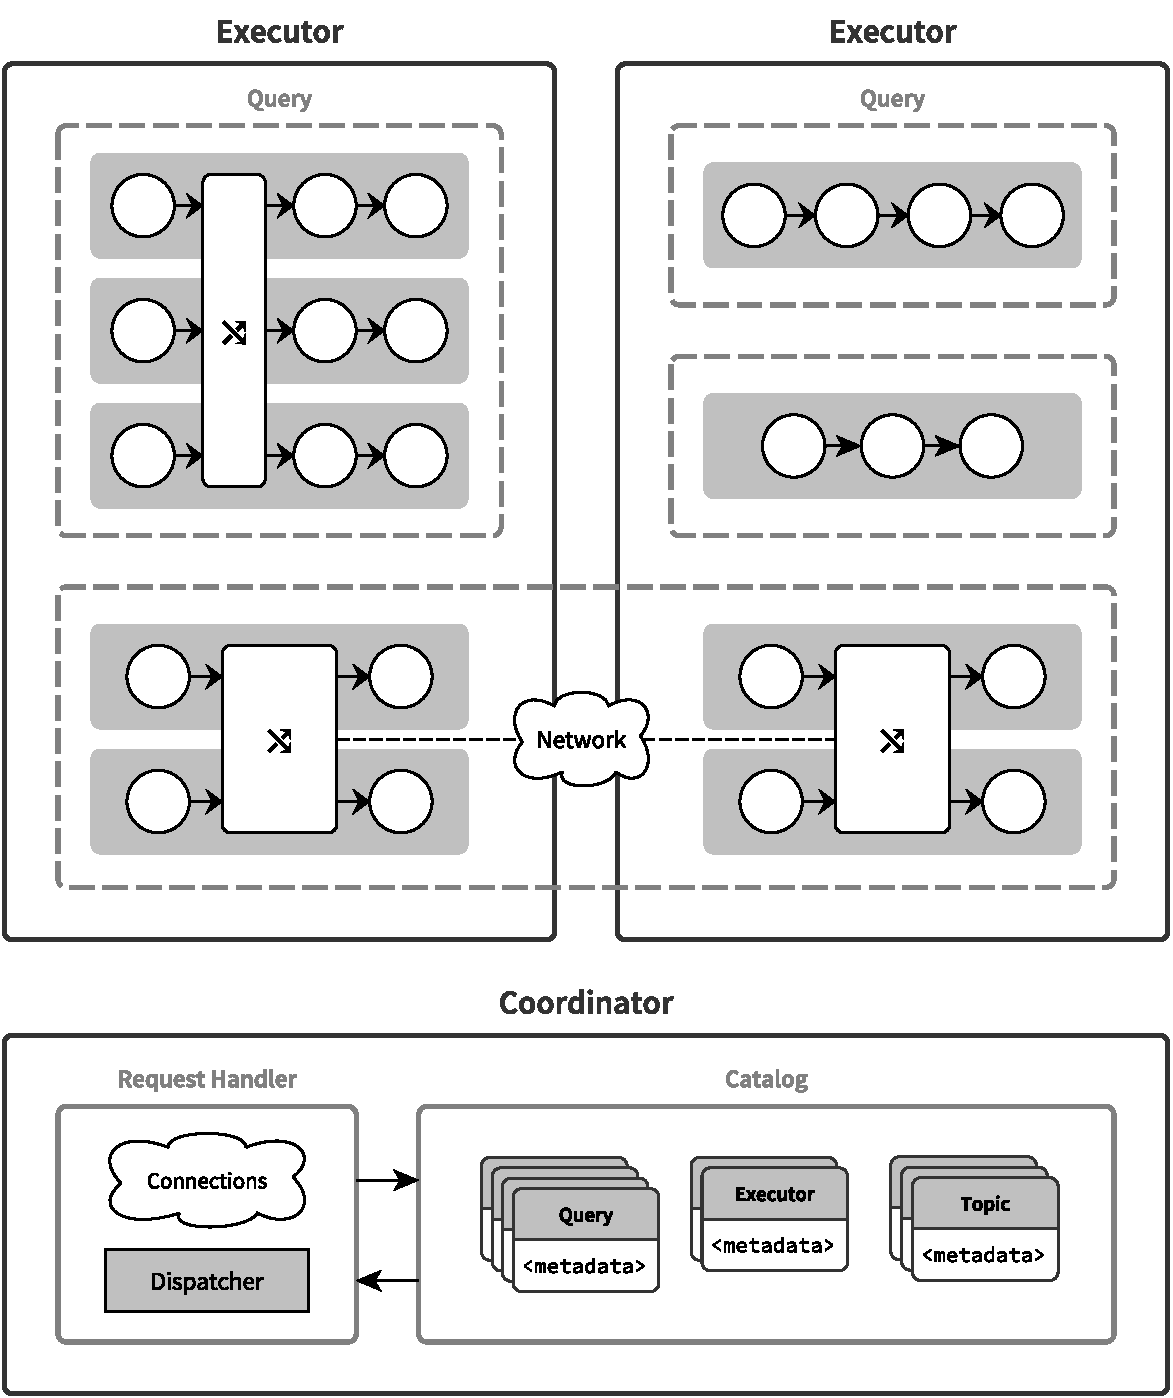
\includegraphics[width=1\textwidth]{figures/components}
  \caption[System architecture.]{ Queries (dashed boxes) consist of one or
  more worker threads (rounded grey boxes) driving the dataflow computation.
  A query might span over multiple executors, make use of the network for message exchanges
  between the workers of a query.\\
  The coordinator maintains a connection to every  executor and every query process.
  The state of the whole system is stored in the catalog.}
  \label{fig:components}
\end{figure}

\clearpage

\section{Queries}

A query is a Timely program managed and executed by our system. Like
standalone Timely Dataflow programs, queries are written in Rust by using the
Timely Dataflow library: The dataflow graph is constructed by connecting
Timely's operators (vertices) to stream objects (edges).

In order for a Timely Dataflow program to become a runnable query on the system,
it needs to register its computational logic with with our system library instead of
using Timely Dataflow's initialization function. This
\lstinline{timely_query::execute} function not only performs the initialization
for the query, it also provides additional functionality to interact with the
coordinator. Other than this, there are no no restrictions on the query program,
it might execute arbitrary code.

\begin{lstlisting}[caption={[Example query.]Example query which creates a stream of integers,
filters out all odd numbers and then prints the rest.}]
extern crate timely;
extern crate timely_query;

use timely::dataflow::Scope;
use timely::dataflow::operators::{Filter, Inspect, ToStream};

fn main() {
    timely_query::execute(|root, catalog| {
        root.scoped::<u32, _, _>(|scope| {
            (0..100).to_stream(scope)
                .filter(|x| x % 2 == 0)
                .inspect(|x| println!("hello {:?}", x));
        });
    }).unwrap();
}
\end{lstlisting}

\subsection{Submission}

A query is submitted to the coordinator as a binary executable. A submission
consists of an URL and format of the query binary, as well as the runtime
configuration for the workers. The runtime configuration specifies the amount
and distribution of the worker threads which will drive the query.

Optionally, a human-readable description of the query,
as well as the command-line arguments to be passed to the executable can be
provided. \TODO{this is currently not implemented}

When handling a new query submission request, the coordinator will assign a
unique identifier to the incoming query, and then select a
matching number of executors for the query to be spawned on. The selection
of executors is based on the runtime configuration provided by the submission
request.

The coordinator plays an important role when spawning new queries. After
issuing query spawn requests to the executors, it waits for all query processes
to register themselves at the coordinator before they begin their computation.
Only then the query is considered active and the submission request
is reported to be completed.

\begin{figure}[htb]
  \centering
    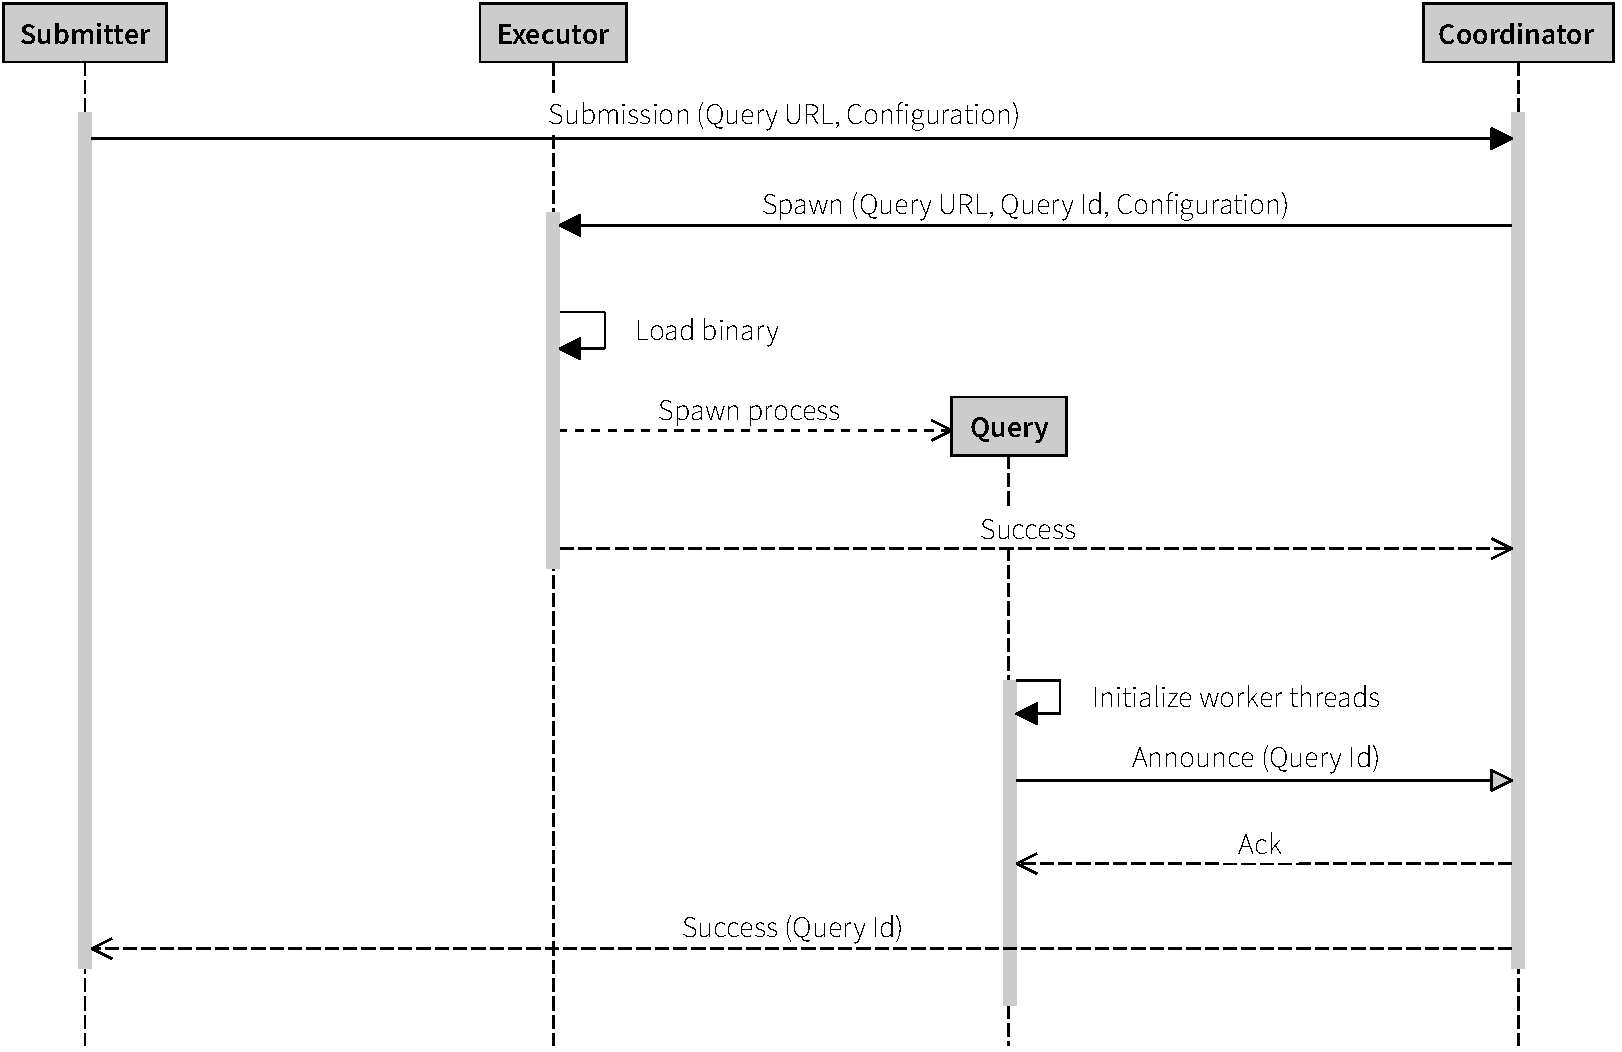
\includegraphics[width=1\textwidth]{figures/spawn_singleprocess}
  \caption[Query submission with single process.]{Submission of a query on a single executor.
  Only once the spawned query announces itself at the coordinator is it considered running.}
  \label{fig:subsingle}
\end{figure}

\section{Executors}

The actual execution and direct supervision of query processes is not done by the
coordinator itself, but is offloaded to designated processes called executors.
This choice allows for more flexibility regarding query execution and the
management of available resources. Since executors can be dynamically be added
to the system, and with some limitations also be removed again, they provide
for instance a way to add new machines to the cluster running our system.

Another feature of executors are that they offer choice on how queries and their
worker threads are supposed to be executed and scheduled. When a executor joins
the system by introducing itself to the coordinator, the executor also informs
the coordinator about the execution format it supports.

In the current implementation, the only supported execution format are native
operating system executables which are spawned as separate processes. However,
alternative executor implementations could for example host multiple queries
within the same process, by dynamically loading the query's code into an already
running process and run it on a preemptive OS thread. This would allow queries
the interchange of objects without the need for data serialization. Given
the implementation of Timely's operator scheduling, cooperative scheduling
of multiple worker threads on a single operating system thread would be
conceivable.

It is also the executors task to fetch query binaries before execution. When
submitting a new query, the submitter provides the coordinator with the URL of
the binary. This URL is forwarded to selected executors, which will use it to
download the query binary.

When spawning a new query, the query process and its executor coordinate:
The executor will supply the newly created process with the information
it needs in order to participate in the system. This includes
the address of the coordinator, the address of any peer processes belonging to the 
same query, the number of worker threads to spawn and the query's own identifier.
Using this information, the query process will spawn its worker threads on behalf
of the executor.

A query might span over multiple executors. The placement of a query on the
available executors is performed by the coordinator, based on the users request.
We currently implement a naive approach to query placement, where the executors
are chosen randomly. A more sophisticated scheduling, which for example could
include load balancing, has to be investigated.

\TODO{Maybe talk about the removal of executors, in the case of OS processes they could
be removed before their queries terminate.}

\section{Exposing data streams}

Dataflow programs often work on streams from external sources. As the same
data source might be processed by multiple dataflow computations, it is
appropriate to manage these streams in our system as well. In some cases, it
might be desirable to perform some preprocessing on the raw data stream.

These assumptions motivate us to extend our system by adding functionality
for queries to expose their data streams for consumption by other queries.
The Timely library already offers the capture and replay for this purpose, where
all timestamp, data and event records are captured in one query, and can then
be replayed in another one.

The implementation of the replay operator requires it to use the same timestamps
as the capture operator, forcing both queries to have a similar structure
in their dataflow graph, as a timestamp received at an operator is defined
by its surrounding scope. Another feature of the capture/replay operator pair
is that they will replay the whole stream from beginning to end, requiring the
capture operator to either buffer its incoming data or wait for the replaying
query to connect to it.

Both these requirements stem from the fact that the replay operator not only
replays the data stream, but also all progress tracking events, including
notifications. In our system, we opted for a more dynamic approach, where
producing queries are allowed to discard data if there are no consumers, and
where consumers use the streams as inputs for their own computation,
allowing them to assign their own timestamps to the data stream.

We loosely adapted the terminology of publish/subscribe systems: Using the
\emph{publish} operator, a query can expose one of its stream
(an edge in the dataflow graph) to other queries, which in turn then \emph{subscribe}
to it. The list of all published topics is stored at in the catalog.

\subsection{Topics}

A topic has the following properties, which are all stored in the catalog
and can be accessed by other queries.
\begin{description}
\item [Identifier] A unique identifier for the topic instance.
\item [Name] When publishing a stream, the publisher has to assign a name to it.
Queries use this name to refer to topics they want to subscribe to. There might
be only one topic with a certain name at a time, however names can be reused if
topics are unpublished.
\item [Data type] A descriptor of the data type published in this topic. Timely's
streams are typed channels, therefore so are topics.
\item [Address] An address to which the subscribers connect in order to received
the contents of the published stream.
\end{description}

While every publication and subscription request is disclosed to the coordinator
and the catalog contains a list of all existing topics, the
actual exchange of data happens directly between queries. When a query subscribes
to a topic, it receives the address of the topic's publisher from the coordinator
and directly connects to it.

\subsection{Publisher}

A publisher is a Timely operator which exposes its input edge as a topic. When
creating it, the query author has to assign a name for the topic under which the
input stream will be published. As with all other Timely operators, the publisher
operator is instantiated on all worker threads. However, the user can choose
whether all worker streams are merged into a single topic before publishing, or
if each worker publishes its own topic. The latter option implicitly exposes
the data sharding strategy of the publishing query, allowing the workers of
the subscribing query to exploit it.

\TODO{Writing this I realized that we probably want to change this, a topic
should be a conceptual stream, which may or may not contain the shared substream.
Subscribers should decide if they want to subscribe to the merged stream, or
just one shard.}

\subsection{Subscriber}

In order to subscribe to a topic, the subscribing query has to provide the name
of the topic it is interested in. This involves a name lookup which can optionally
be blocking: If a requested topic does not yet exist, the coordinator will add
the subscriber to a wait list. Once a corresponding topic is published under that
name, the coordinator will inform the subscriber about this topic. 

The subscribing query might use different timestamps in its dataflow graph
than the publisher, thus it is the subscribers responsibility to re-add
timestamps to the received stream. 

\TODO{The story with multiple worker threads in the subscribing query is
not really clear as well.}



